Having studied the spatial error in detail, we next study the temporal error and the requisite timestep to achieve a certain accuracy across both algorithms. 
\subsubsection{Floren's data}
We begin with an analysis of Floren's data. Again, the ``exact'' solution is Floren's fiber evolution for $\tilde{N}=24$, $\Delta t =10^{-6}$ (the finest spatial and temporal discretization provided). Fig.\ \ref{fig:FN12} shows the $L^2$ errors for $\tilde{N}=12$ and a variety of timesteps for Floren's algorithm. We observe the $L^2$ errors in Floren's algorithm for $\tilde{N}=12$ are more or less saturated by the spatial error. Even for a timestep as small as $10^{-6}$, there is still an $L^2$ error of $\mathcal{O}(10^{-2})$. 

Given the large spatial error, it remains to be seen what timestep Floren has to use to get a temporal error less than or equal to the spatial error for $\tilde{N}=12$. As shown in Fig.\ \ref{fig:FN12temp}, a timestep of $\Delta t =10^{-3}$ gives an $L^2$ difference of $\approx 0.015$ from the evolution when $\Delta t =10^{-6}$. Given that the spatial error is $\approx 0.01$, we conclude that \textbf{Floren can use a $\Delta t =10^{-3}$ for $\tilde{N}=12$ and get a temporal error less than or equal to the spatial error}. 

\begin{figure}
\centering 
\subfigure[``Error'' wrt $\tilde{N}=24$]{
\label{fig:FN12}
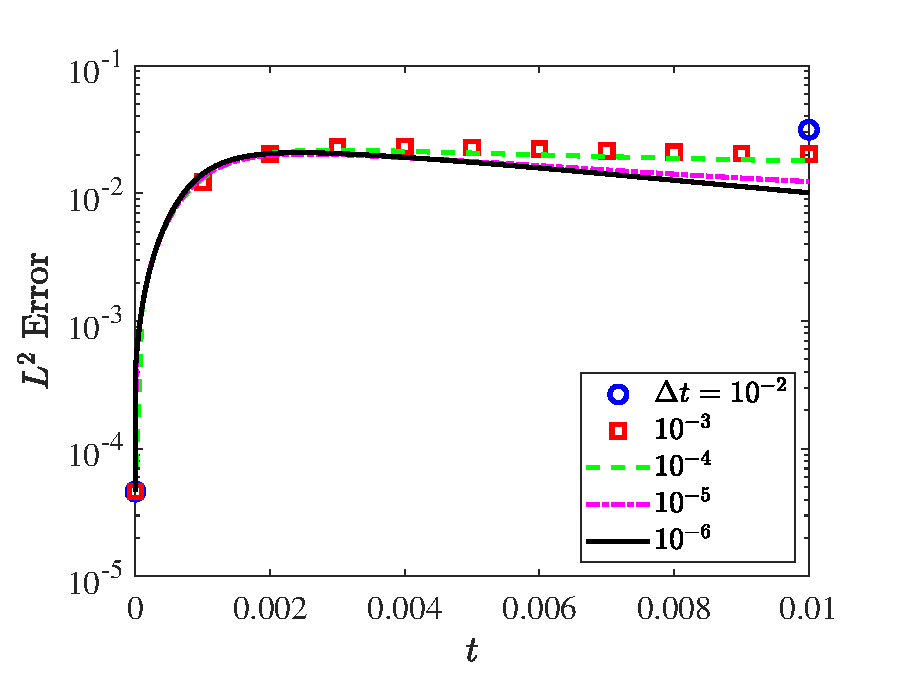
\includegraphics[width=70mm]{FlorenTemporalN12.eps}}
\subfigure[``Error'' wrt $\tilde{N}=12$]{
\label{fig:FN12temp}
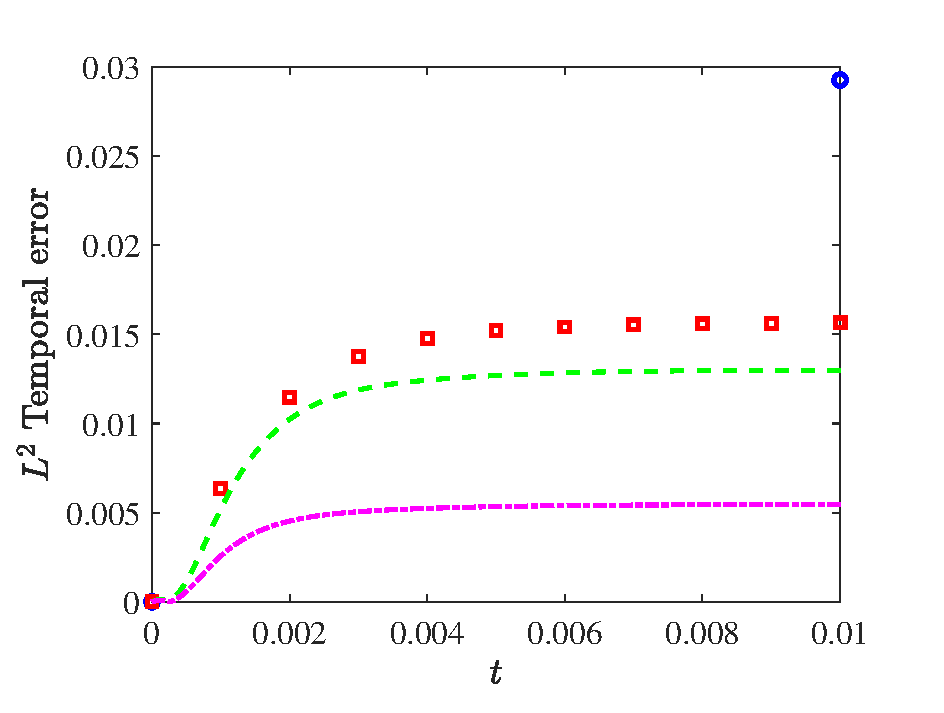
\includegraphics[width=70mm]{FlorenN12Temporal.eps}}
\caption{(a) $L^2$ errors over time when comparing to Floren's ``exact'' solution with $\tilde{N}=24$, $\Delta t=10^{-6}$ to his solutions when $\tilde{N}=12$. (b) $L^2$ \textit{temporal} errors in Floren's algorithm for $\tilde{N}=12$ using $\tilde{N}=12$ $\Delta t = 10^{-6}$ as the ``exact'' solution. Timesteps are color coded as blue circles ($10^{-2}$), red squares ($10^{-3}$), dashed green lines ($10^{-4}$), dashed-dotted pink lines ($10^{-5}$), and solid black lines ($10^{-6}$). } 
\label{fig:Flortemp}
\end{figure}

\subsubsection{Accuracy of temporal integration for fixed spatial discretization}
\label{sec:rk3fe}
We next focus on our algorithm with a fixed spatial discretization. For simplicity and ease of running multiple simulations, we choose $N=8$. We first check the order of accuracy of the SSP RK3 scheme
\begin{gather}
\bm{X}^{n+1} = \bm{X}^n + \Delta t \left(\frac{1}{6}\bm{k}_1 + \frac{1}{6}\bm{k}_2+\frac{2}{3}\bm{k}_3\right)\\[4 pt]
\bm{k}_1 = \bm{u}\left(\bm{X}^n\right) \qquad \bm{k}_2 = \bm{u}\left(\bm{X}^n + \Delta t \bm{k}_1\right) \qquad \bm{k}_3 = \bm{u}\left(\bm{X}^n + \frac{\Delta t}{4} \bm{k}_1 + \frac{\Delta t}{4} \bm{k}_2\right).
\end{gather}
Importantly, for this test we will use successive refinements to measure convergence (rather than comparing to Floren's results). As shown in Fig.\ \ref{fig:RK3N8}, SSP RK3 is a third order accurate scheme, as the errors scale as $\Delta t^3$. Importantly, the temporal error for $\Delta t = 10^{-4}$ using RK3 is $10^{-5}$, which is 2 orders of magnitude less than the spatial error of $10^{-3}$ (see Fig.\ \ref{fig:L2}). Furthermore (this data is not shown on the plot), using $\Delta t = 2 \times 10^{-4}$ gives a maximum $L^2$ error of $9 \times 10^{-5}$ and $\Delta t = 4 \times 10^{-4}$ gives a maximum $L^2$ error of $2 \times 10^{-2}$ in RK3. 

Next, we take the solution from SSP RK3 with $\Delta t =10^{-6}$ and treat this (which has converged to 12 digits) as an exact solution for $N=8$. We seek the error from forward Euler. The timestep $\Delta t =10^{-3}$ is unstable. As shown in Fig.\ \ref{fig:FEN8}, using a timestep half of this unstable $\Delta t$ yields a large error. However, for $\Delta t =10^{-4}$ and lower, we see the expected first order convergence. Furthermore, 4 digits of accuracy are observed for $\Delta t =10^{-4}$. Finally (this data is not shown on the plot), using $\Delta t = 2 \times 10^{-4}$ gives a maximum $L^2$ error of $6 \times 10^{-4}$ and $\Delta t = 4 \times 10^{-4}$ gives a maximum $L^2$ error of $4 \times 10^{-2}$ in forward Euler. \textbf{Therefore, the conclusion is that there is no reason to use RK3 in this scheme. While the temporal accuracy is slightly improved in RK3, the $10^{-3}$ spatial error still dominates for every $\Delta t \leq 2 \times 10^{-4}$, regardless of whether forward Euler or RK3 is used. Put another way, for any $\Delta t$ for which the temporal error is less than or equal to the spatial error, forward Euler is sufficient.}

\begin{figure}
\centering 
\subfigure[SSP RK3]{
\label{fig:RK3N8}
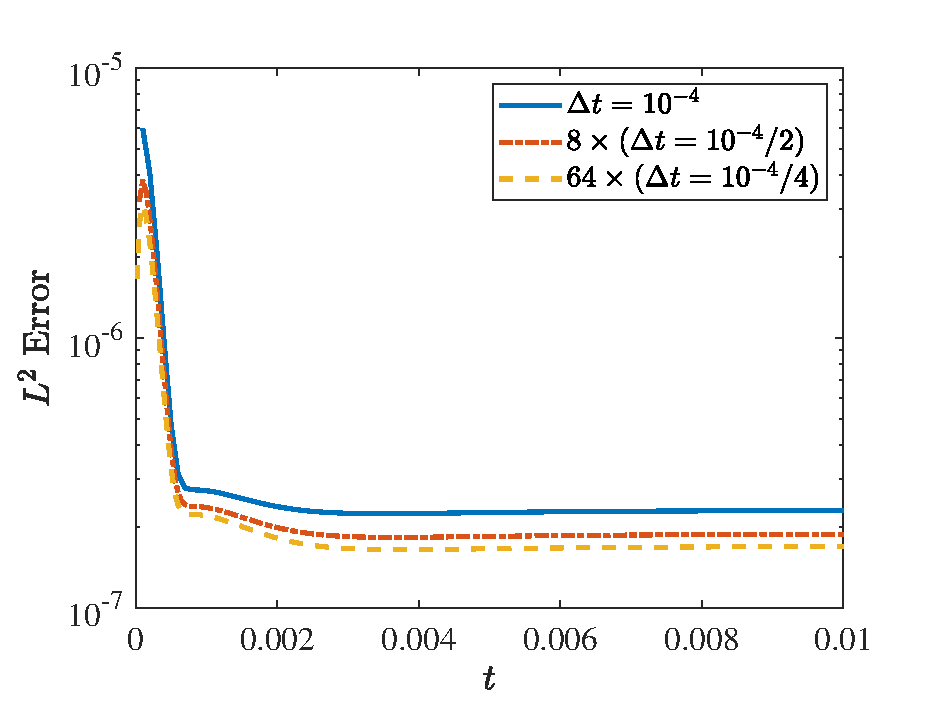
\includegraphics[width=70mm]{RK3N8.eps}}
\subfigure[Forward Euler]{
\label{fig:FEN8}
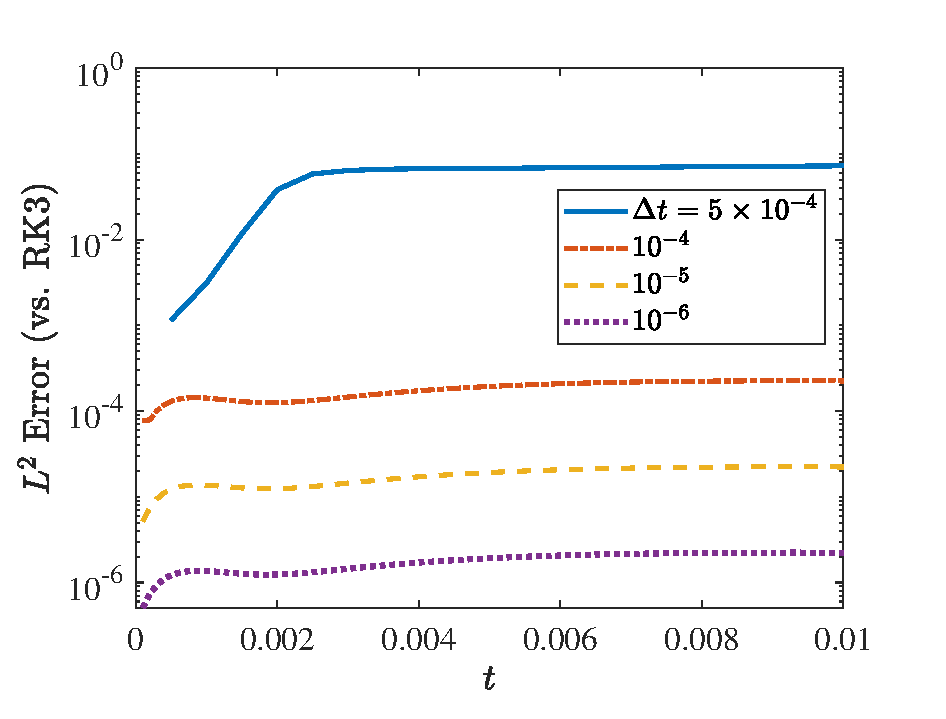
\includegraphics[width=70mm]{FEErrorN8.eps}}
%\subfigure[Our explicit scheme]{
%\label{fig:UsEx}
%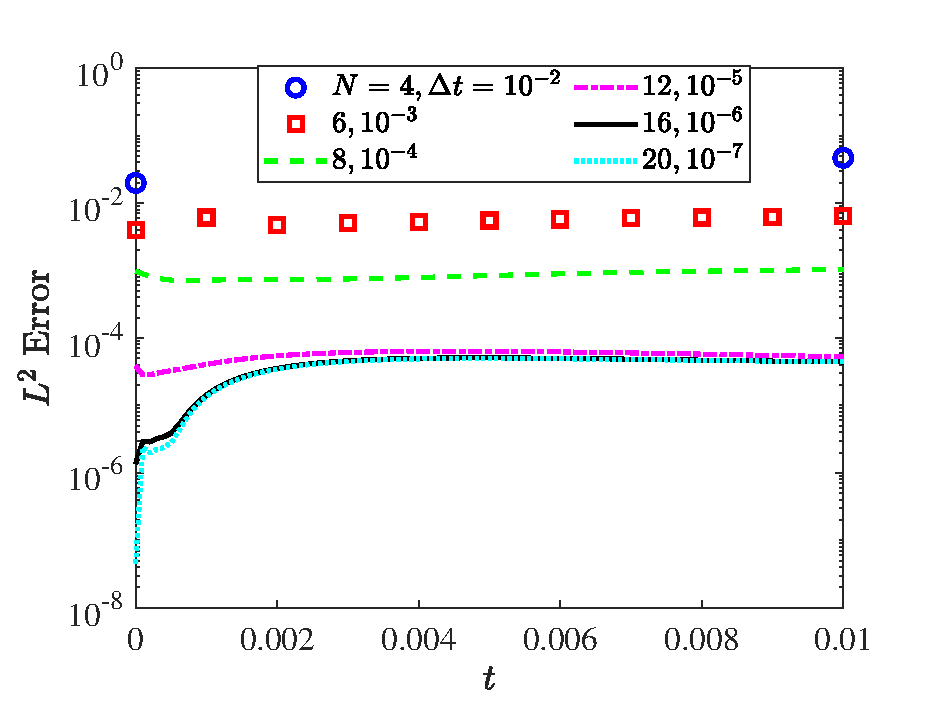
\includegraphics[width=70mm]{UsTemporalSpatial.eps}}
\caption{Temporal accuracy for a fixed spatial discretization $N=8$. (a) $L^2$ error for SSP RK3 on $N=8$ (with respect to successive refinements in $\Delta t$ by a factor of 2). The error for $\Delta t =10^{-4}$ (blue line) is approximately 8 times the error for $\Delta t = 10^{-4}/2$ (dashed/dotted red line) and 64 times the error for $\Delta t =10^{-4}/4$. The scheme is therefore third-order accurate. (b) Accuracy of the forward Euler method when compared to the ``exact solution'' from SSP RK3. $\Delta t = 5 \times 10^{-4}$ (blue line) is clearly inaccurate; it is likely too close to the stability limit. $\Delta t=10^{-4}$ (dashed/dotted red), $\Delta t =10^{-5}$ (dashed yellow), and $\Delta t =10^{-6}$ (dotted purple) demonstrate first order convergence starting at an $L^2$ error of $10^{-4}$. We conclude that the first-order method is sufficient since temporal error is less than spatial error for any $\Delta t \leq 2 \times 10^{-4}$.} 
\end{figure}

\subsubsection{Spatio-temporal accuracy of our scheme}
Since we cannot choose any timestep, we seek some kind of comparison between our method and Floren's. That is, a way to compare to Fig.\ \ref{fig:Flortemp}. We therefore set up the following experiment: consider spatial discretizations from $N=6, 8, \dots 20$. We run the \textit{forward Euler} temporal integrator with \textit{the first stable timestep that is a power of 10}. The accuracy of this temporal integration is verfied by ensuring the maximum $L^2$ error in time is of the same order of magnitude with a $\Delta t$ that is half the relevant power of 10. 

For this section, we return to using Floren's maximally refined evolution as the ``exact'' solution (i.e. the same ``exact'' solution as in Fig.\ \ref{fig:FN12}). 

Shown in Fig.\ \ref{fig:UsEx} is the overall accuracy of our scheme under spatio-temporal refinement. \textbf{In our case, a timestep of $10^{-4}$ is stable up to $N=8$ points, and we get an accuracy of $10^{-3}$. This is an order of magnitude better than Floren, whose errors are spatially dominated for this $\Delta t$. Furthermore, for $\Delta t = 10^{-3}$, (when Floren's spatial and temporal errors are comparable) we still get higher accuracy with $N=6$ than Floren with $\tilde{N}=12$!}



\begin{figure}
\centering 
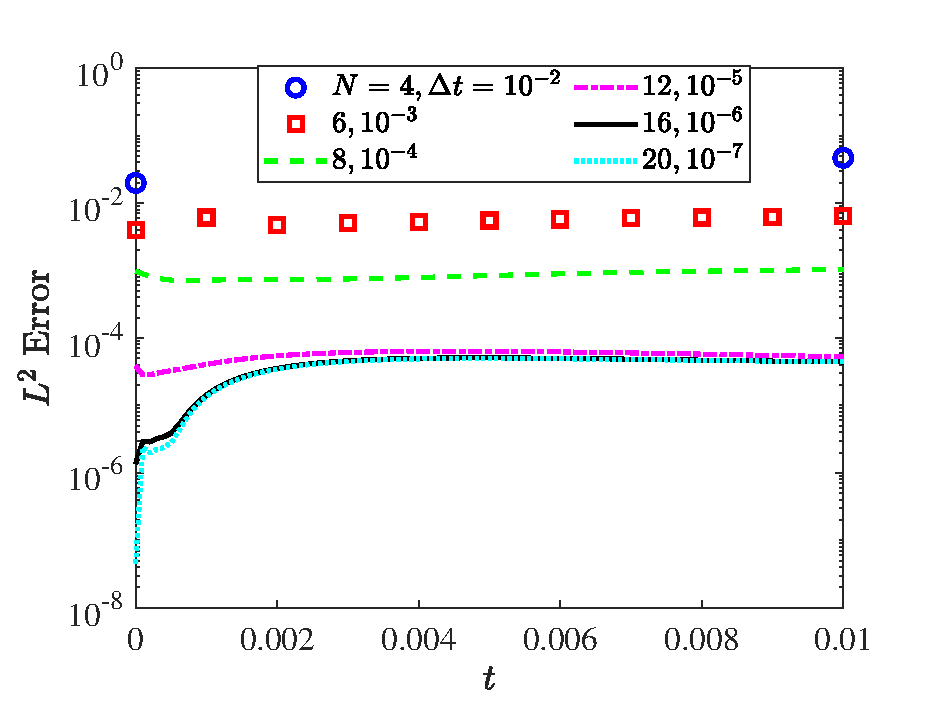
\includegraphics[width=70mm]{UsTemporalSpatial.eps}
\caption{Overall spatio-temporal accuracy of our scheme. Timestep is the first stable power of 10 using forward Euler integration for a given spatial discretization. Recall that the relative error in displacement is approximately 10 times the $L^2$ error. } 
\label{fig:UsEx}
\end{figure}

\subsection{Implicit timestepping}
\subsubsection{Backward Euler}
We recall that we can define $\bm{f}^E = \bm{L}\bm{X}$ on the type 1 grid. With this in mind, we can write the equations for a backward Euler update as
\begin{gather}
\label{eq:tup}
\bm{X}^{n+1} = \bm{X}^{n} + \Delta t  \bm{K} \bm{\alpha} \\[2 pt]
\label{eq:BEeqn}
\bm{K}\bm{\alpha}= \bm{M}^n\left(\bm{\lambda}+\left(\bm{f}^E\right)^{n+1}\right)+\bm{U}_0^{n+1}\\[2 pt]
\bm{K}^* \bm{\lambda}=\begin{pmatrix} \bm{0}\\[2 pt] -\bm{I}^*\left(\bm{f}^E\right)^{n+1}\end{pmatrix}
\end{gather}
Now suppose that $\bm{U}_0$ is a time-dependent linear function of $\bm{X}$ (in our experiments it will be). Then we write (by abuse of notation) $\bm{U}_0^{n+1} = \bm{U}_0^{n+1}\bm{X}^{n+1}$. 
Eq.\ \eqref{eq:tup} can then be used to rewrite these equations in block form as
\begin{equation}
\label{eq:impsolve}
\bm{A}\bm{y}=
    \begin{pmatrix}
    -\bm{M} &\bm{K}-\Delta t \bm{MLK}-\Delta t \bm{U}_0^{n+1}\bm{K} \\[4 pt]
   \bm{K}^* &\begin{pmatrix} \bm{0}\\[2 pt]\Delta t \bm{I}^*\bm{LK}\end{pmatrix} 
    \end{pmatrix}^n
    \begin{pmatrix} 
    \bm{\lambda}\\[4 pt]
    \bm{\alpha}\\[4 pt]
    \end{pmatrix} =  \begin{pmatrix} 
   \bm{ML}\bm{X}^n+\bm{U}_0^{n+1}\bm{X}^n\\[4 pt]
    \begin{pmatrix} \bm{0}\\[4 pt]
    -\bm{I}^*\bm{L}\bm{X}^n \end{pmatrix}
    \end{pmatrix}. 
\end{equation}

The matrices $\bm{M}$ and $\bm{K}$ depend on $\bm{X}$, and these are treated explicitly. The bending force $\bm{f}^E = \bm{L}\bm{X}$ is always treated implicitly. Note that this results in an $(5N+1)^2$ linear system, which is exactly the same size as in the explicit case, Eq.\ \eqref{eq:saddlept}. 

Now, we saw in Section \ref{sec:space} that the $L^2$ spatial error of our discretization is $\approx 10^{-3}$. However, in Fig.\ \ref{fig:FEN8}, we saw that temporal error near the boundary of the stability region is $10^{-4}$. If we used a larger timestep than $\Delta t = 1-2 \times 10^{4}$, we saw ballooning errors. In this section, we ask whether we can ``fix'' this with implicit timestepping. 

Table \ref{tab:imp} shows the ``savings'' when using backward Euler for different $N$. All of the errors are the maximal $L^2$ error over time. The first column is the spatial error, which is the difference between an RK3 simulation (accurate to 10 digits) of the given $N$ and an RK3 simulation of $N=20$ (which we take as the exact solution). Our goal is for the temporal error, which is the difference between a given ($N$,\, $\Delta t$) pair and the ``exact'' RK3 solution for the same $N$, to be on the same order as the spatial error. Table \ref{tab:imp} shows what timestep is necessary for this.

Considering $N=4$ and $N=8$, we see that the forward Euler method is limited by stability and we can get a savings by switching to backward Euler. For $N > 8$, the spatial discretization is converging so rapidly that we are limited by accuracy; and forward Euler and backward Euler get the same result. So it appears that backward Euler is not particularly advantageous (at least for this very smooth problem), except for $N=8$ when we get a factor of 5. 


%\begin{figure}
%\centering 
%\subfigure[Temporal Errors]{
%\label{fig:tempImp}
%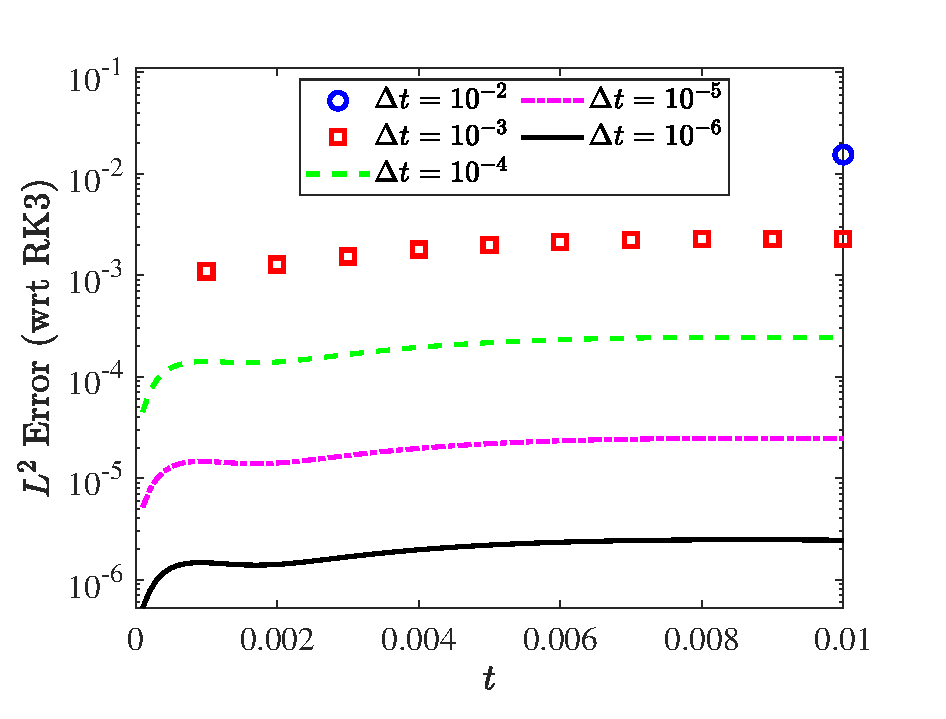
\includegraphics[width=70mm]{ImplicitRK3Er.eps}}
%\subfigure[Spatio-temporal Errors]{
%\label{fig:STImp}
%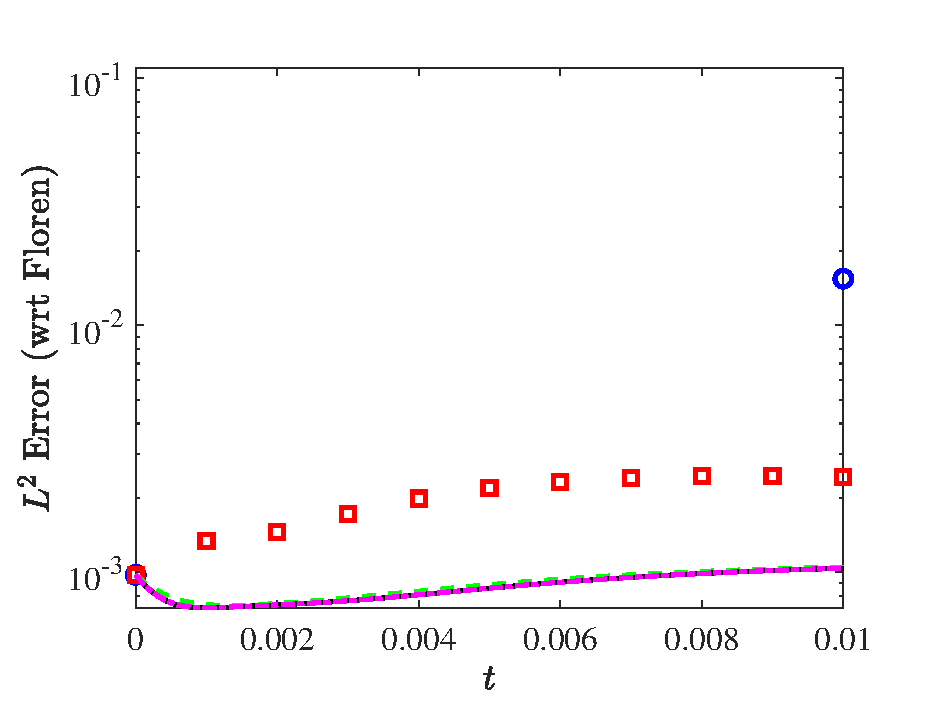
\includegraphics[width=70mm]{ImplicitFlorenEr.eps}}
%\caption{Effect of implicit time-stepping on spatio-temporal error. (a) $L^2$ error over time when comparing with the explicit RK3 solution (known to be accurate to 10 digits). The time integrator is first order, and we can get an $L^2$ error of $\approx 2 \times 10^{-3}$ by taking $\Delta t =10^{-3}$, previously impossible due to stability. Color scheme is the same as Fig. \ref{fig:Flortemp}. (b) Total $L^2$ error using Floren's maximally refined solution as the exact solution. Any timestep $\leq 10^{-4}$ isolates the $10^{-3}$ spatial error. $\Delta t =10^{-3}$ gives an ideal balance of spatial and temporal error.} 
%\end{figure}

\begin{table}
\centering
\begin{tabular}{c|c|c|c|c|c|c|c} 
$N$ & Spatial Er & FE $\Delta t$ &  FE Temp Er & BE $\Delta t$ & BE Temp Er & CN $\Delta t$ & CN Temp Er \\
\hline
4 & 2.23e-2 & $5 \times 10^{-3}$ & 1.35e-2 & $10^{-2}$ & 1.98e-2 &  $10^{-2}$ & 1.28e-2\\[2 pt]
8 & 1.04e-3 & $2 \times 10^{-4}$ & 5.60e-4 & $10^{-3}$ & 2.29e-3 &  $2 \times 10^{-3}$ & 1.58e-3\\[2 pt]
12 & 3.83e-5 & $10^{-5}$ & 2.23e-5&  $10^{-5}$ & 2.47e-5 &  $2 \times 10^{-4}$ & 2.69e-5\\[2 pt]
16 & 2.32e-6 &  $10^{-6}$ & 2.23e-6& $10^{-6}$ & 2.48e-6 &  $5 \times 10^{-5}$ & 1.72e-6
\end{tabular}
\caption{Comparing the required timestep to match the spatial error (measured against $N=20$ RK3) with the temporal error (measured against the RK3 spatial solution for that $N$) using  forward Euler (FE), backward Euler (BE), and Crank-Nicolson (CN). All errors are maximum $L^2$ errors over time. }
\label{tab:imp}
\end{table}

\subsubsection{Crank-Nicolson}
We combine Crank-Nicolson with a linear multi-step method to obtain a second-order scheme with one solver per timestep. Specifically, we set
\begin{equation}
\label{eq:LMM}
\bm{X}^{n+1/2. *} = \frac{3}{2}\bm{X}^n - \frac{1}{2}\bm{X}^{n-1}.
\end{equation}
We then solve 
\begin{equation}
\label{eq:CNsolve}
\bm{A}\bm{y}=
    \begin{pmatrix}
    -\bm{M} &\bm{K}-\frac{1}{2}\Delta t \bm{MLK} -\frac{1}{2}\Delta t \bm{U}_0^{n+1}\bm{K}\\[4 pt]
   \bm{K}^* &\begin{pmatrix} \bm{0}\\[2 pt]\frac{1}{2}\Delta t \bm{I}^*\bm{LK}\end{pmatrix} 
    \end{pmatrix}^{n+1/2, *}
    \begin{pmatrix} 
    \bm{\lambda}\\[4 pt]
    \bm{\alpha}\\[4 pt]
    \end{pmatrix} =  \begin{pmatrix} 
   \bm{ML}\bm{X}^n+\frac{1}{2}\left(\bm{U}_0^{n}+\bm{U}_0^{n+1}\right)\bm{X}^n\\[4 pt]
    \begin{pmatrix} \bm{0}\\[4 pt]
    -\bm{I}^*\bm{L}\bm{X}^n \end{pmatrix}
    \end{pmatrix}.
\end{equation}
Eq.\ \eqref{eq:CNsolve} is now the system to be solved at every timestep, with the operators $\bm{M}$ and $\bm{K}$ evaluated using Eq.\ \eqref{eq:LMM}. Because we saw that backward Euler gave little to no savings over forward Euler, our goal in this section is to determine whether a \textit{second-order} implicit scheme (which requires one solve per timestep) gives a savings over an explicit one. 
 
Fig.\ \ref{fig:FECN} shows that the Crank-Nicolson scheme is second-order accurate and gives a much lower temporal error for $\Delta t \leq 10^{-3}$ than backward Euler for $N=8$. Furthermore, we see in Table \ref{tab:imp} that the Crank-Nicolson temporal update can give a temporal error comparable to the spatial error for much larger timesteps than forward/backward Euler. In particular, for $N=4, 8, 12$, and 16, we see a savings from Crank-Nicolson (over forward Euler) that is a factor of 1, 10, 20, and 50. This comes at no extra cost (other than a possibly dangerous extrapolation step), since we are doing a $(5N+1)^2$ least squares solve once per timestep in all cases. 

\begin{figure}
\centering 
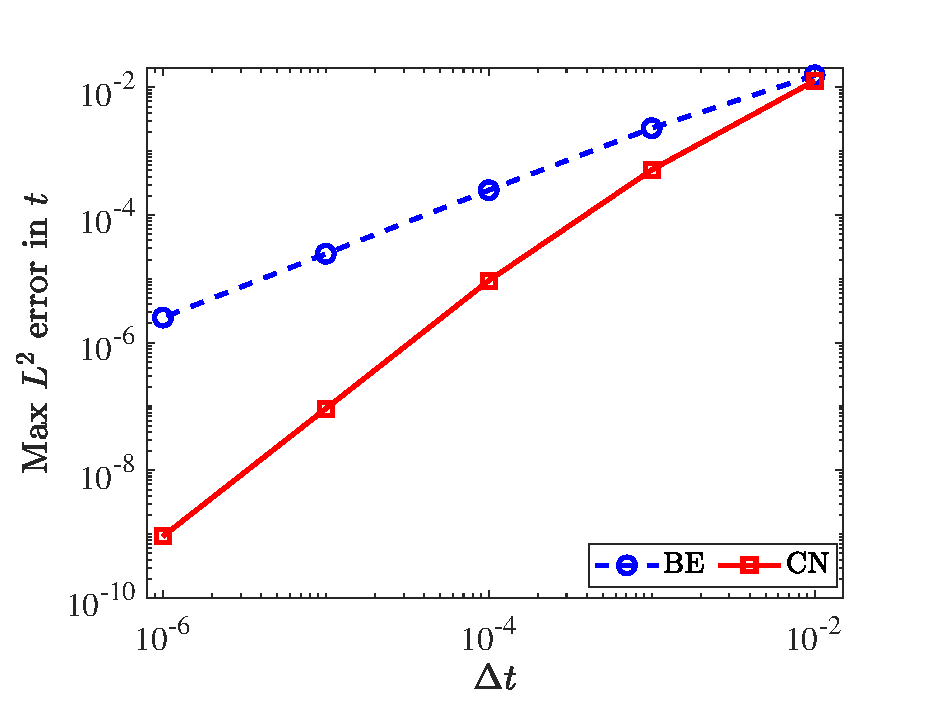
\includegraphics[width=70mm]{FECN.eps}
\caption{Comparing the temporal error from backward Euler (red circles) and Crank-Nicolson (blue squares) for $N=8$. Shown is the maximum $L^2$ error (wrt the RK3 explicit solution accurate to 10 digits) over time for different $\Delta t$. First order convergence is observed for backward Euler, and second-order convergence is observed for Crank-Nicolson. Table \ref{tab:imp} has more details on the savings that can be obtained for different $N$.  } 
\label{fig:FECN}
\end{figure}